\newpage
\begin{slikaDesno}{fig/proc_1.pdf}[fig/proc_2.pdf]
    \noindent
    \textbf{{\color{red}*}\ID.}
    На слици \ID.1 jе представљена принципска шема система за
    генерисање и довођење сигнала такта до одговараjућег прикључка
    дигиталног процесора. Генератор такта jе идеалан напонски
    генератор симетричне униполарне поворке правоугаоних импулса
    учестаности
    $f_{\rm clk} = \dfrac{1}{T_{\rm clk}} = 4\unit{MHz}$
    и амплитуде $V_{\rm m} = 5\unit{V}$. 
    Линиjа за пренос такта моделуjе се као као каскадна
    веза идеалног блока за кашњење, кашњења 
    $\uptau = 125\unit{ns}$, и идеаланог филтра пропусника ниских учестаности,чиjа
    jе фреквенциjска преносна карактеристика 
    $H(\jj\upomega) = \rect\left( \dfrac{\upomega}{2\upomega_0} \right)$, где је 
    $\upomega_0$ непознати параметар. 
    Према спецификациjи употребљеног процесора, при
    преласку напона такта са ниског на високи ниво, дозвољено jе
    да у прелазноj зони између $V_1 = 1,5\unit{V}$ и $V_2 = 3,5\unit{V}$, доведени сигнал такта
    проведе наjвише 
    $\Delta t_{\rm max} = 5\unit{ns}$, као што jе илустровано на слици \ID.2. 
    \end{slikaDesno}

    (а) Одредити развоjе генерисаног сигнала такта, $v_{\rm clk}(t)$, и сигнала такта
    на улазу у процесор $v_{\rm clk}^{\rm(CPU)}(t)$ у комплексан Фуријеов ред у зависности 
    од параметра $\upomega_0$.
    (б) Одредити коефицијенте развоја сигнала $\dfrac{\de v_{\rm clk}^{\rm (CPU)}(t)}{\de t}$ 
    у комплексан Фуријеов ред.  
    (в) Одредити параметар $\upomega_0$ тако да буде задовољена наведена спецификација датог 
    процесора. 

    \underline{\it Напомена.} Приликом прорачуна времена које сигнал такта проводи у 
    прелазној зони, претпоставити да је нагиб сигнала такта 
    $\dfrac{\de v_{\rm clk}^{\rm (CPU)}(t)}{\de t}$ практично константан и да има максималну 
    вредност. \\

    \textsc{\underline{Решење}}: Генерисани сигнал такта јесте периодична поворка правоугаоних импулса. 
    Спектар такве поворке, на основном периоду $T_{\rm clk}$, на основу резултата задатка 
    \ref{ID:rect_pulse_train_FS} је $V_{\rm clk}[k] = 
    (-\jj)^k \dfrac{V_{\rm m}}{2} \sinc \left(
    \dfrac{k}{2}
    \right) $.
    Модел линије за пренос сачињен је из каскадне везе идеалног филтра и линије за 
    кашњење $T[k] = \rect \left( \dfrac{k{\upomega_{\rm clk}}}{2\upomega_0} \right) 
    \cdot \ee^{-\jj k {\upomega_{\rm clk}\uptau}} = 
    \rect \left( \dfrac{k{\upomega_{\rm clk}}}{2\upomega_0} \right) 
    \cdot (-1)^k$. Спектар напона на улазу у процесор онда је коначног облика 
    \begin{equation}
        V_{\rm clk}^{\rm (CPU)}[k] 
        = T[k] \cdot V_{\rm clk}[k] 
        =  
        \dfrac{\jj^{k} V_{\rm m}}{2}
        \rect \left( \dfrac{k{\upomega_{\rm clk}}}{2\upomega_0} \right) 
        \cdot
        \sinc \left(
        \dfrac{k}{2} \right)
    \end{equation}

    (б) Применимо правило извода\footnote{Правило извода је 
    $
    \mathcal{FS}\left\{\dfrac{\de x(t)}{\de t}\right\} = \jj k \upomega_{\rm 0} 
    \mathcal{FS}\left\{ x(t) \right\} $ \\[1mm]} добија се резултат
    \begin{equation}
        \FS{ \dfrac{v_{\rm clk}^{\rm (CPU)}}{\de t}} [k]
        = 
        \dfrac{ 
        \jj^{k+1} \,
        k \upomega_{\rm clk} \, 
        V_{\rm m} }{2}
        \rect \left( \dfrac{k{\upomega_{\rm clk}}}{2\upomega_0} \right) 
        \cdot
        \sinc \left(
        \dfrac{k}{2} \right)
    \end{equation}

    (в) 
    Због симетрије, током преласка кроз средину прелазне зоне, сигнал има максималан нагиб у тренутку 
    $t = \uptau$, будући да је и ивица сигнала за толико закашњена. По претпоставци из напомене 
    са таквим нагибом нагибом треба да пређе целу прелазну зону за највише време 
    $\Delta t_{\rm max}$. Односно треба да важи
    \begin{equation}
        \dfrac{ v_{\rm clk}^{\rm (CPU)} }{\de t} (\uptau) > \dfrac{\Delta V}{\Delta t_{\rm max}}
        = 0,4\unit{\dfrac{V}{ns}}  \label{eq:\ID.uslov}
    \end{equation}

    Вредност извода у том тренутку потражује се на основу синтетичке релације\footnote{
    Користи се у облику $x(\uptau) = \sum_{k = -\infty}^{\infty} X[k] \ee^{\jj k\upomega_{\rm F} \uptau}$
    } Фуријеовог реда као 
    \begin{align}
        \dfrac{v_{\rm clk}^{\rm (CPU)}}{\de t}  (\uptau)
        =& 
        \sum_{k = \infty}^{\infty} 
        \FS{ \dfrac{v_{\rm clk}^{\rm (CPU)}}{\de t} }[k] \, \ee^{\jj k \upomega_{\rm clk} \uptau} 
        = 
        \FS{ \dfrac{v_{\rm clk}^{\rm (CPU)}}{\de t} }[k] \, (-1)^k \\[1.5mm]
        =&
        \sum_{k = \infty}^{\infty} 
        \dfrac{ 
        (-1)^k \jj^{k+1} k \upomega_{\rm clk} \, 
        V_{\rm m} }{2}
        \rect \left( \dfrac{k{\upomega_{\rm clk}}}{2\upomega_0} \right) 
        \cdot
        \sinc \left(
        \dfrac{k}{2} \right). \label{eq:\ID.dvtau}
    \end{align}
    За израчунавање суме распишимо да је 
    $k \sinc\dfrac{k}{2} = 
    \cancel{k} \dfrac{\sin\left( \frac{k\uppi}{2} \right) }{ \frac{\cancel{k}\uppi}{2} }
    $, те приметимо да је \linebreak
    ${\sin\left( \frac{k\uppi}{2} \right) = 
    \begin{cases}
        (-1)^m ,&  k = 2m+1 \\
        0      ,& k = 2m
    \end{cases}}$. Заменом добијених резултата  
    у $\eqref{eq:\ID.dvtau}$ и сређивањем помоћу 
    $ (-1)^k \jj^{k+1} \bigg|_{k = 2m+1} = 
    (-1)^{2m + 1} \jj^{2m + 2} = (-1)^m
    $
    ,има се 
    $
        \dfrac{v_{\rm clk}^{\rm (CPU)}}{\de t}  (\uptau)
        = \DS
        \sum_{\substack{ k = -\infty \\ k = 2m + 1 } }^{\infty} 
        \dfrac{ 
        \upomega_{\rm clk} \, 
        V_{\rm m} }{\uppi}
        \rect \left( \dfrac{{k \upomega_{\rm clk}}}{2\upomega_0} \right)  
    $. Вечичина под сумом је парна функција па се може одговарајућа\footnote{
        Трансформација за парни сигнал $a[k]$ је 
        $\sum_{k = -\infty}^{\infty} a[k] = a[0] + 2\sum_{k = 1}^{\infty} a[k]$.
    }
    трансформација. Добијена сума се онда може
    може средити изражавањем правоугаоног импулса у облику
    $
        \rect \left( \dfrac{{k \upomega_{\rm clk}}}{2\upomega_0} \right)
        =
        \begin{cases}
            1,& k < \dfrac{\upomega_{\rm 0}}{\upomega_{\rm clk}} \\[5mm]
            0,& k > \dfrac{\upomega_{\rm 0}}{\upomega_{\rm clk}} 
        \end{cases}
    $, што се може искористити за постављање горње границе коначне суме:
    $
        \dfrac{v_{\rm clk}^{\rm (CPU)}}{\de t}  (\uptau)
        = \DS
        \sum_{\substack{ k = -\infty \\ k = 2m + 1 } }^{k < \upomega_0 / \upomega_{\rm clk} } 
        \dfrac{ 2
        \upomega_{\rm clk} \, 
        V_{\rm m} }{\uppi} 
    $. Број чланова добијене суме јесте $М$, број непарних бројева између $0$ и 
    $\dfrac{\upomega_0}{\upomega_{\rm clk}}$, а који има смисао   
    броја непарних хармоника сигнала такта које пропушта филтар.  
    \\[2mm]
    
    
    Одавде се има 
    $\dfrac{\de v_{\rm clk}^{\rm (CPU)}}{\de t} (\uptau)
    = 
    M
    \dfrac{ 2
        \upomega_{\rm clk} \, 
        V_{\rm m} }{\uppi} 
    $, на основу услова из \eqref{eq:\ID.uslov}, заменом бројевних вредности налази се услов 
    за број непарних хармоника које филтар треба да пропусти. Одавде се има услов да је 
    $M = 
    \dfrac{\uppi} { 2
        \upomega_{\rm clk} \, 
        V_{\rm m} } 
    \dfrac{\de v_{\rm clk}^{\rm (CPU)}}{\de t} (\uptau)
    > 12,5 \unit{\dfrac{ns}{V}} \cdot 0,4 \unit{\dfrac{nV}{s}} = 5$. Односно, филтар мора да пропусти
    \textit{барем} 5 \textit{непарних} хармоника побудног сигнала, а то су
    $\upomega_{\rm clk}$, $3\upomega_{\rm clk}$, $5\upomega_{\rm clk}$, $7\upomega_{\rm clk}$, и
    $9\upomega_{\rm clk}$, односно, мора бити да је 
    $\upomega_0 > 9\upomega_{\rm clk}$, или 
    $f_0 > 9f_{\rm clk} = 36\unit{MHz}$.    
 
    У овом задатку је илустровано, да је стримина ивице правоугаоних импулса сразмерна
    броју хармоника које пропушта филтар. На слици \ID.3 илустрован је резултат. 
    Црвеним областима обележени су габарити унутар којих сигнал не сме да пролази, 
    односно назначене су границе прелазне зоне по времену и по напону. Нацртани су сигнали 
    са 1--5 непарних хармоника, и на слици може да се види да су са најмање 5
    непарних хармоника задовољени
    тражени габарити. 

    \begin{figure}[ht!]
        \centering
        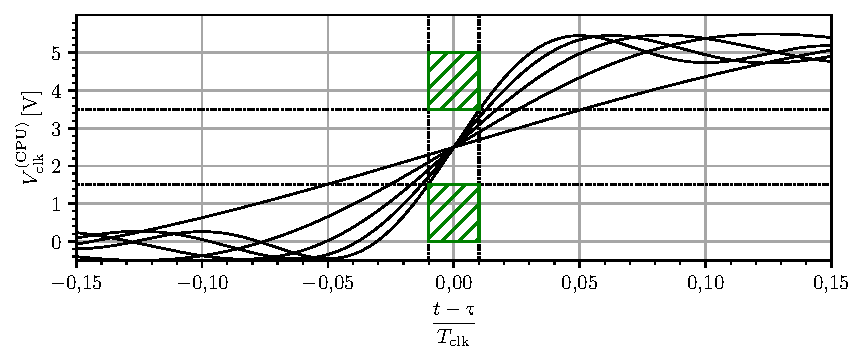
\includegraphics[scale=1]{fig/proc_plot.pdf} 
        \caption{}
    \end{figure}